\section{Itération~3:~(~4/3/2017~-~4/28/2017~)}
\subsection{Introduction}
\subsection{L'objectif du sprint}
En accord avec le product owner,le but de cette itération est:
\begin{itemize}
 \item \textbf{Smart phone :}L’ajout de nouvelles fonctionnalités comme :
        \begin{itemize}
         \item La détection des réseaux avec leur intensité.
         \item l'exploitation des donnes collecté selon le besoin.
        \end{itemize}
\item \textbf{Rapport :} Typage des rapports.
\item \textbf{Dashboard :}
        \begin{itemize}
         \item Élaboration des mécanisme d'authentification.
         \item Des nouveaux marqueurs qui spécifient chaque type de rapport ajouté.
        \end{itemize}

\end{itemize}

%Le Product Owner nous a demandé d’améliorer le chargement de l'image
%dans le serveur de telle sorte que la qualité d'image reste la même..
%Donc, dans cette itération, nous allons tenir compte des attentes du Product Owner. Nous allons
%modifier le critère de chargement, En plus nous allons implémenter une méthode
%permettant de maintenir la qualité.

\subsection{Planification de l'itération 3}

\subsubsection{Backlog de l'itération}

Le but de cette itération est d'ajouter un système de gestion des rapport et d'améliorer
la qualité.

\begin{center}
    \footnotesize
    \begin{longtable}{| p{1cm} | p{5cm} | p{7cm} | p{1cm} |}
        \caption{Taches à faire de la troisième itération}
        \label{tab:sprint3-backlog} \\

 \hline
 \multicolumn{1}{|c}{\textbf{Réf}} &
 \multicolumn{1}{|c}{\textbf{Spécification}} &
 \multicolumn{1}{|c}{\textbf{Description}} &
 \multicolumn{1}{|c|}{\textbf{Priorité}} \\ \hline
 \endhead

 \hline \multicolumn{4}{|r|}{{Continué en page suivante$\dotsc$}} \\ \hline
 \endfoot

 \hline \hline
 \endlastfoot

\hline
1 & Integration Dashboard et Rapport dans l'application android & Implémenté la méthode qui affiche les pages ``Dashboard et Rapport'' chacun a un bouton spécifié   & 1 \\ \hline
2 & Authentification Restful  & Ajouter l'authentification dans le serveur pour assurer la sécurité   & 1 \\ \hline
3 & landing page & créer une nouvel page Web  & 3\\ \hline
4 & Compte utilisateur & Base de données accecible depuis l'application et le web& 2 \\ \hline
5 & Post réseau & Methode POST Restful & 1 \\ \hline
6 & GET réseau & Methode GET Restful & 1 \\ \hline
7 & Post vitesse & Methode POST vitesse & 1 \\ \hline
8 & Get vitesse & Methode GET & 1 \\ \hline
9 & Appplication Android Responsive & Responsive design coter android & 3 \\ \hline
10 & IHM & l'ajout des boutons radio pour distinguer (pieton / voiture)(android) & 3 \\ \hline
11 & Recherche Business intelligence & BI & 2 \\ \hline
12 & Implantation des BD au BI & données accessible en BI & 2\\ \hline
13 & création Logo &Ajouter Logo dans l'application & 3 \\ \hline
14 & étude scénario commercial embouteillage & scénario de marketing& 2\\ \hline
15 & Rectification chargement image & \ldots & 1 \\ \hline
16 & étude scénario commercial secousses & scénario de marketing& 2\\ \hline
\end{longtable}
\end{center}

\subsubsection{Estimation de la deuxième itération}
\begin{table}[htbp]
    \centering
    \begin{tabular}{| c | c | c | c |}
\hline
\textbf{Membre} & \textbf{Nombre d'heures par jour} & \textbf{Nombre de jours présent} & \textbf{Total en heures} \\ \hline
\hline

Moez & 8 & 48 & 144\\ \hline
Rihab & 8 & 48 & 144 \\ \hline
\multicolumn{2}{c|}{} & \textbf{Total} & 288 \\ \cline{3-4}
    \end{tabular}
    \caption{Nombre d'heures de travail estimé de l'itération 3}
    \label{tab:sprint3-capacity}
\end{table}

\begin{center}
    \begin{longtable}{| l | l | l |}
        \caption{Nombre d'heures estimé pour la réalisation des taches}
        \label{tab:sprint3-estimation} \\

 \hline
 \multicolumn{1}{|c}{\textbf{Spécification}} &
 \multicolumn{1}{|c}{\textbf{Membre}} &
 \multicolumn{1}{|c|}{\textbf{Heures}} \\ \hline
 \endhead

 \hline \multicolumn{3}{|r|}{{Continué en page suivante$\dotsc$}} \\ \hline
 \endfoot

 \hline \hline
 \endlastfoot

\hline
Integration Dashboard et Rapport dans l'application android & Rihab & 5 x 2 \\ \hline
Authentification Restful& Rihab & 5 x 2 \\ \hline
landing page& Rihab & 5 x 2 \\ \hline
Compte utilisateur& Rihab & 5 x 2 \\ \hline
Post réseau& Rihab & 5 x 2 \\ \hline
GET réseau& Rihab & 5 x 2 \\ \hline
Post vitesse& Rihab & 5 x 2 \\ \hline
Get vitesse& Rihab & 5 x 2 \\ \hline
Appplication Android Responsive & Rihab & 5 x 2 \\ \hline
IHM & Rihab & 5 x 2 \\ \hline
Recherche Business intelligence& Rihab & 5 x 2 \\ \hline
Implantation des BD au BI& Rihab & 5 x 2 \\ \hline
création Logo& Rihab & 5 x 2 \\ \hline
Étude scénario commercial embouteillage& Rihab & 5 x 2 \\ \hline
Rectification chargement image & Rihab & 5 x 2 \\ \hline
Étude scénario commercial secousses & Rihab & 5 x 2 \\ \hline
\end{longtable}
\end{center}

\subsection{Présentation des outils utilisés}
\subsubsection{API REST}
Les API REST sont basées sur le protocole HTTP, qui signifie Hypertext Transfer Protocol.
C’est ce qui est au cœur du web! C’est un protocole qui définit la communication
entre les différentes parties du web. L’échange est basé sur des requêtes client et serveur.
Un client lance une requête HTTP, et le serveur renvoie une réponse.
Ce sont des méthodes qui définissent les requêtes que le client peut effectuer,
dont GET\footnote{Récupérer une ressource (ne modifie pas la ressource).}, PUT\footnote{Modifier une ressource.},
POST\footnote{Créer une ressource.}, DELETE\footnote{Supprimer une ressource.} encore plus.

\subsubsection{Business Intelligence}

la Business intelligence\footnote{Informatique décisionnelle} propose d'utiliser
les données transitant par le Système
d'information, données de production le plus souvent, en informations susceptibles
d'être exploitées à des fins décisionnelles.

Sur le plan pratique et technique, la Business Intelligence se compose d'une famille
d'outils informatiques et
de progiciels assurant le fonctionnement de la chaîne de traitement de l'information.

Les 4 fonctions de la chaîne décisionnelle comment s'explique la figure~\ref{fig:sprint3-businessintelligence} sont:
\begin{description}[align=right,labelwidth=1cm]
 \item [1] Collecter, nettoyer et consolider les données Extraire les données
 des systèmes de production et les adapter à un usage décisionnel.
 \item [2] Stocker Centraliser les données structurées et traitées afin qu'elles
 soient disponibles pour un usage décisionnel.
 \item [3] Distribuer Ou plutôt faciliter l'accessibilité des informations selon
 les fonctions et les types d'utilisation.
 \item [4] Exploiter ou comment assister du mieux possible l'utilisateur afin qu'il puisse extraire
 la substance de l'information des données stockées à cet usage.
\end{description}
\clearpage

\begin{figure}[htbp]
  \centering
  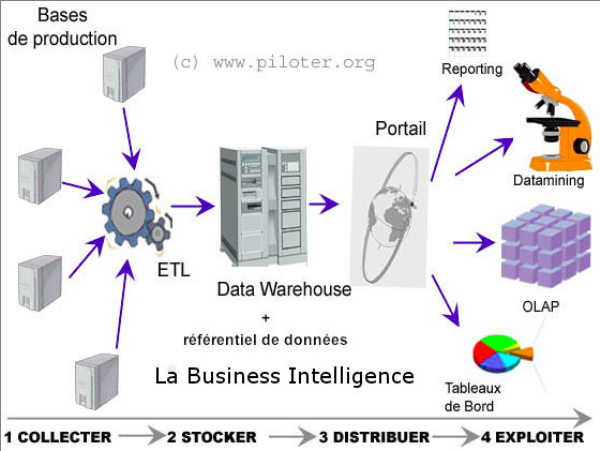
\includegraphics[width=0.8\textwidth]{sprint3-businessintelligence}
  \caption{Les 4 phases du processus de Business Intelligence}
  \label{fig:sprint3-businessintelligence}
\end{figure}


\subsection{Mises des normes}

\subsection{Modélisation UML}

\subsection{Évaluation suivant les normes mise}
\clearpage
\subsection{Revue de cette itération}
On rappelons que nous travaillons dans un équipe Scrum qui nécessite 
l'intégration de notre travail dans le projet pour attentes le but.
\subsubsection{Produit de l'itération}
\paragraph{Légende du Dashboard}
Dans cette page nous travaillons alors sur deux parties:
\begin{itemize}
 \item la première : active/désactive les bouton des filtrages de chaque marqueur.
 \item la deuxième : gérés la communication interne entre serveur et la page .
 \end{itemize}
Aussi,nous participons 80\% à l'ajout de légende a notre carte
et afficher le filtrage des marqueurs.\\

\begin{figure}[htbp]
  \centering
  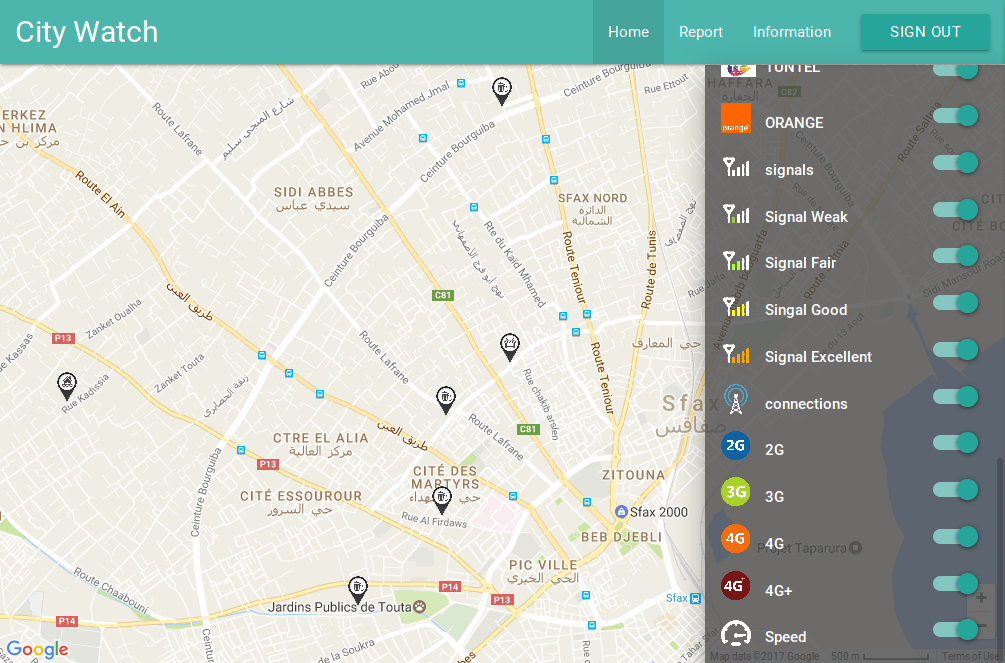
\includegraphics[width=0.8\textwidth]{sprint3-dashboard-screenshot1}
  \caption{Dashboard CityWatch au troisième itération}
  \label{fig:sprint3-dashboard-screenshot1}
\end{figure}
\clearpage
\paragraph{Android}
\paragraph*{}
Les données captées par l'application mobile (Position , Secousses , Ralentisseur , Réseaux , force du 
signal et vitesse ) sont Récupérées par le serveur pour assurer la sauvegarde et la transmission vers une 
base données.\\

\begin{figure}[htbp]
    \begin{subfigure}{.5\textwidth}
    \centering
  \centering
  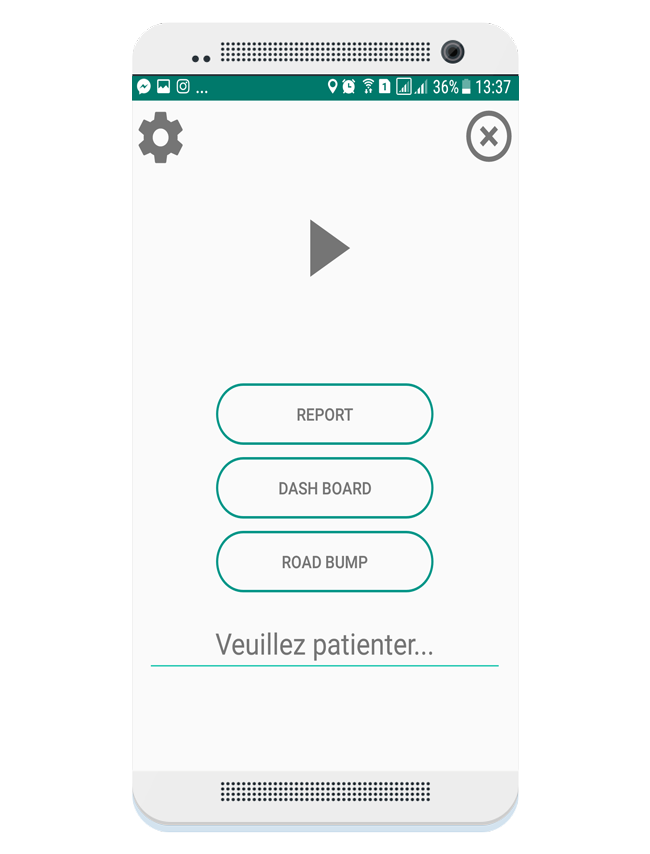
\includegraphics[width=.8\linewidth]{sprint3-android-screenshot1}
  \caption{État désactivé}
  \label{fig:sprint3-android-screenshot1}
\end{subfigure}
\begin{subfigure}{.5\textwidth}
    \centering
  \centering
  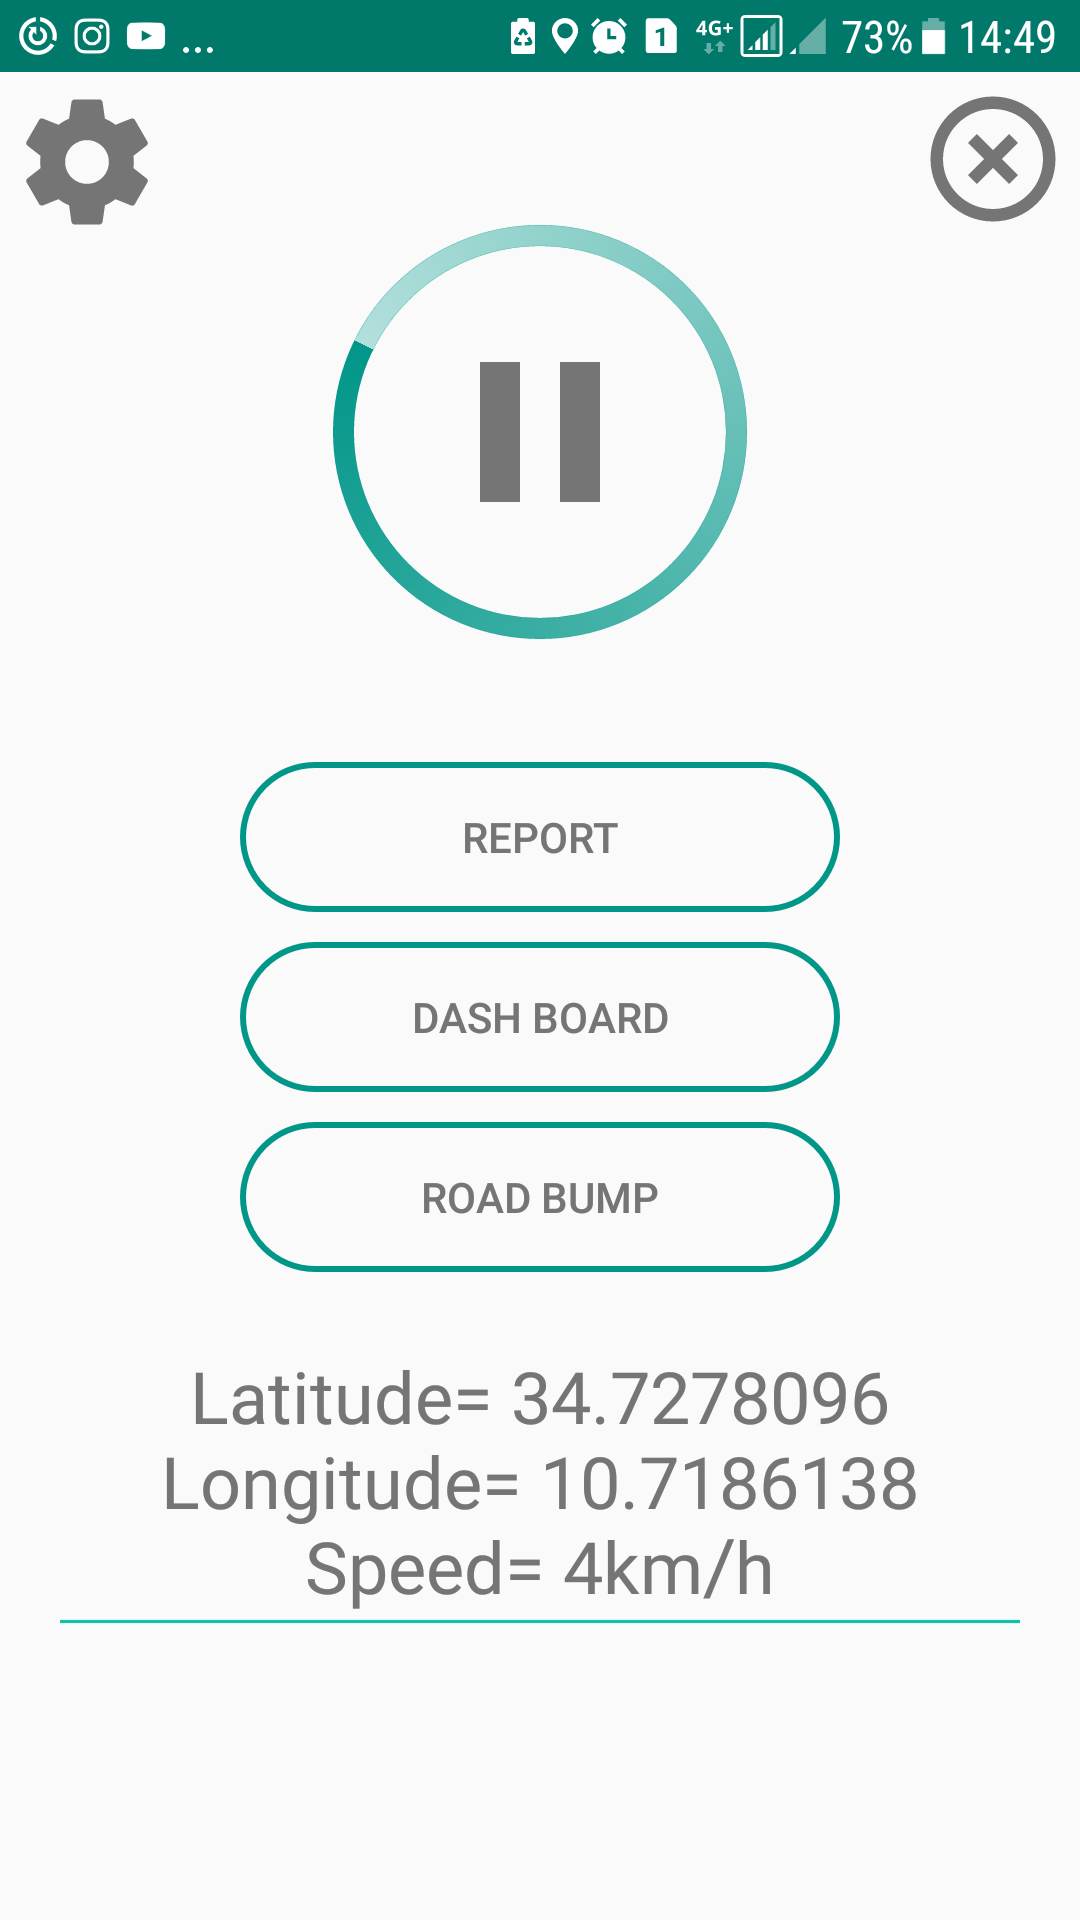
\includegraphics[width=.8\linewidth]{sprint3-android-screenshot2}
  \caption{État activé}
  \label{fig:sprint3-android-screenshot2}
\end{subfigure}
\caption{Interface de l'application au troisième itération}
\end{figure}
\clearpage

\subsubsection{Avis du Product Owner}

Après la présentation du produit final, le \textquote{Product Owner} était très satisfait
a notre travail.

\subsubsection{Graphique d'avancement de l'itération}

\usetikzlibrary{plotmarks}

\begin{figure}
\centering
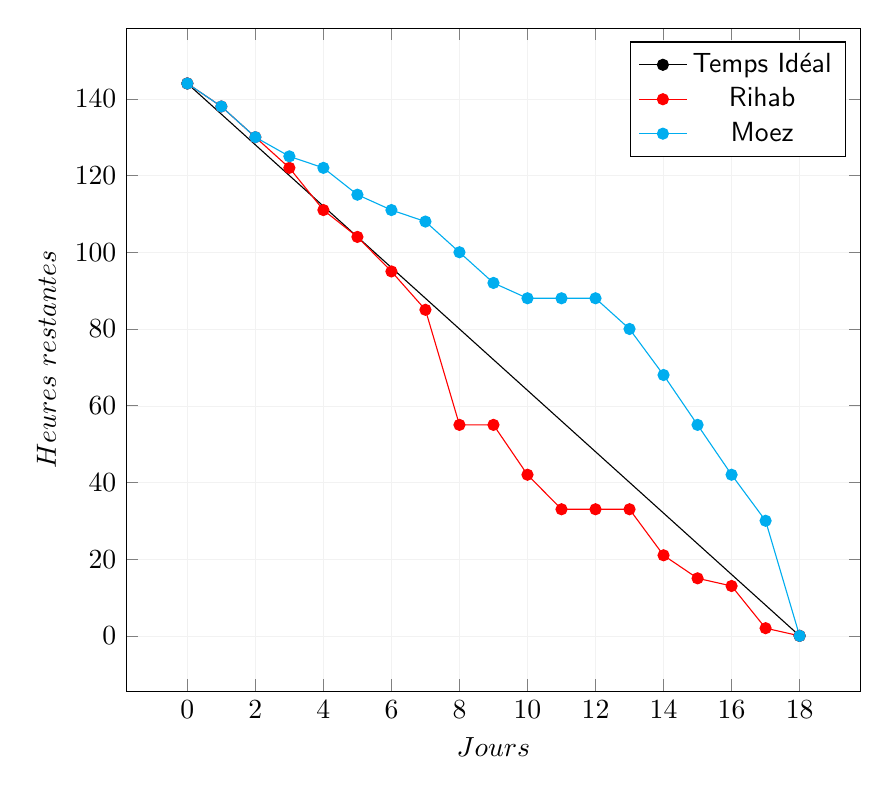
\begin{tikzpicture}[y=.2cm, x=.7cm,font=\sffamily]
\begin{axis}[
xlabel=$Jours$,
ylabel=$Heures\ restantes$,
grid=both,
grid style={line width=.1pt, draw=gray!10},
width=0.9\textwidth,
height=10cm,
%major grid style={line width=.2pt,draw=gray!50},
]
\addplot[color=black,mark=*] coordinates {
        (0,144)
        (18,0)
    };
    \addlegendentry{Temps Idéal}

    \addplot[mark=*,red] plot coordinates {
        (0, 144)
        (1, 138)
        (2, 130)
        (3, 122)
        (4, 111)
        (5, 104)
        (6, 95)
        (7, 85)
        (8, 55)
        (9, 55)
        (10, 42)
        (11, 33)
        (12, 33)
        (13, 33)
        (14, 21)
        (15, 15)
        (16, 13)
        (17, 2)
        (18, 0)
       
    };
    \addlegendentry{Rihab}
      \addplot[mark=*,cyan] plot coordinates {
       (0, 144)
        (1, 138)
        (2, 130)
        (3, 125)
        (4, 122)
        (5, 115)
        (6, 111)
        (7, 108)
        (8, 100)
        (9, 92)
        (10, 88)
        (11, 88)
        (12, 88)
        (13, 80)
        (14, 68)
        (15, 55)
        (16, 42)
        (17, 30)
        (18, 0)
       
    };
    \addlegendentry{Moez}
\end{axis}
\end{tikzpicture}
\caption{Graphique d'avancement - Itération 3}
\end{figure}

\subsection{Conclusion}

\begin{center}
    \begin{longtable}{| l | l |}
        \caption{Liste des tâches réalisées de la troisième itération}
        \label{tab:sprint3-estimation} \\

        \hline
        \textbf{Les tâches} & \textbf{Taux de réalisation} \\ \hline
        \endhead

        \hline \multicolumn{2}{|r|}{{Continué en page suivante$\dotsc$}} \\ \hline
        \endfoot

        \hline \hline
        \endlastfoot

        \hline
Integration Dashboard et Rapport dans l'application android & Effectué 100\% \\ \hline
Authentification Restful&  Effectué 100\% \\ \hline
landing page& Effectué 100\% \\ \hline
Compte utilisateur& Effectué 100\% \\ \hline
Post réseau& Effectué 100\% \\ \hline
GET réseau&  Effectué 100\% \\ \hline
Post vitesse&  Effectué 100\% \\ \hline
Get vitesse& Effectué 100\% \\ \hline
Appplication Android Responsive & Effectué 100\% \\ \hline
IHM & Effectué 100\% \\ \hline
Recherche Business intelligence& Effectué 100\% \\ \hline
Implantation des BD au BI & Effectué 100\% \\ \hline
création Logo&  Effectué 100\% \\ \hline
Étude scénario commercial embouteillage& Effectué 100\% \\ \hline
Rectification chargement image & Effectué 100\% \\ \hline
Étude scénario commercial secousses &  Effectué 100\% \\ \hline
\end{longtable}
\end{center}
